\section{Manage your OS configuration}
\subsection{How container works}

\begin{frame}{Example of R and package installation}{OS virtualisation}
\begin{columns}
\column{.5\textwidth}
\begin{itemize}
	\item "Trick" applications into believing that they are in a different OS than the host’s 
\includegraphics[width=0.2\textwidth]{images/docker_logo2.png}
	\item Avoid redundancy
	\item Speed
	\begin{itemize}
		\item Faster installation
		\item No boot time
	\end{itemize}
	\item Lightweight
	\begin{itemize}
		\item Minimal base OS
		\item Minimal set of library and global environment 
		\item Easy sharing of application 
	\end{itemize}	
\end{itemize}
\column{.5\textwidth}
\begin{itemize}
	\item No easy use on a cluster system
	\item Docker private company policies
\end{itemize}
\end{columns}
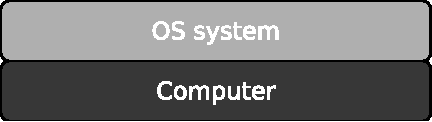
\includegraphics[width=0.1\textwidth]{images/docker_env_1.pdf} 
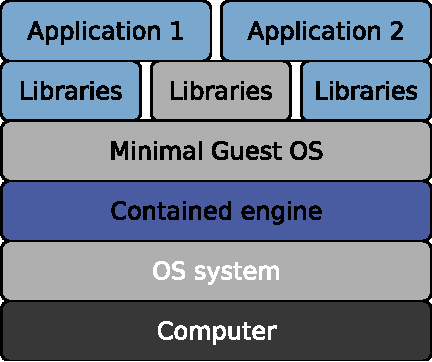
\includegraphics[width=0.1\textwidth]{images/docker_env_2.pdf} 

\includegraphics[width=0.1\textwidth]{images/singularity_logo.pdf}
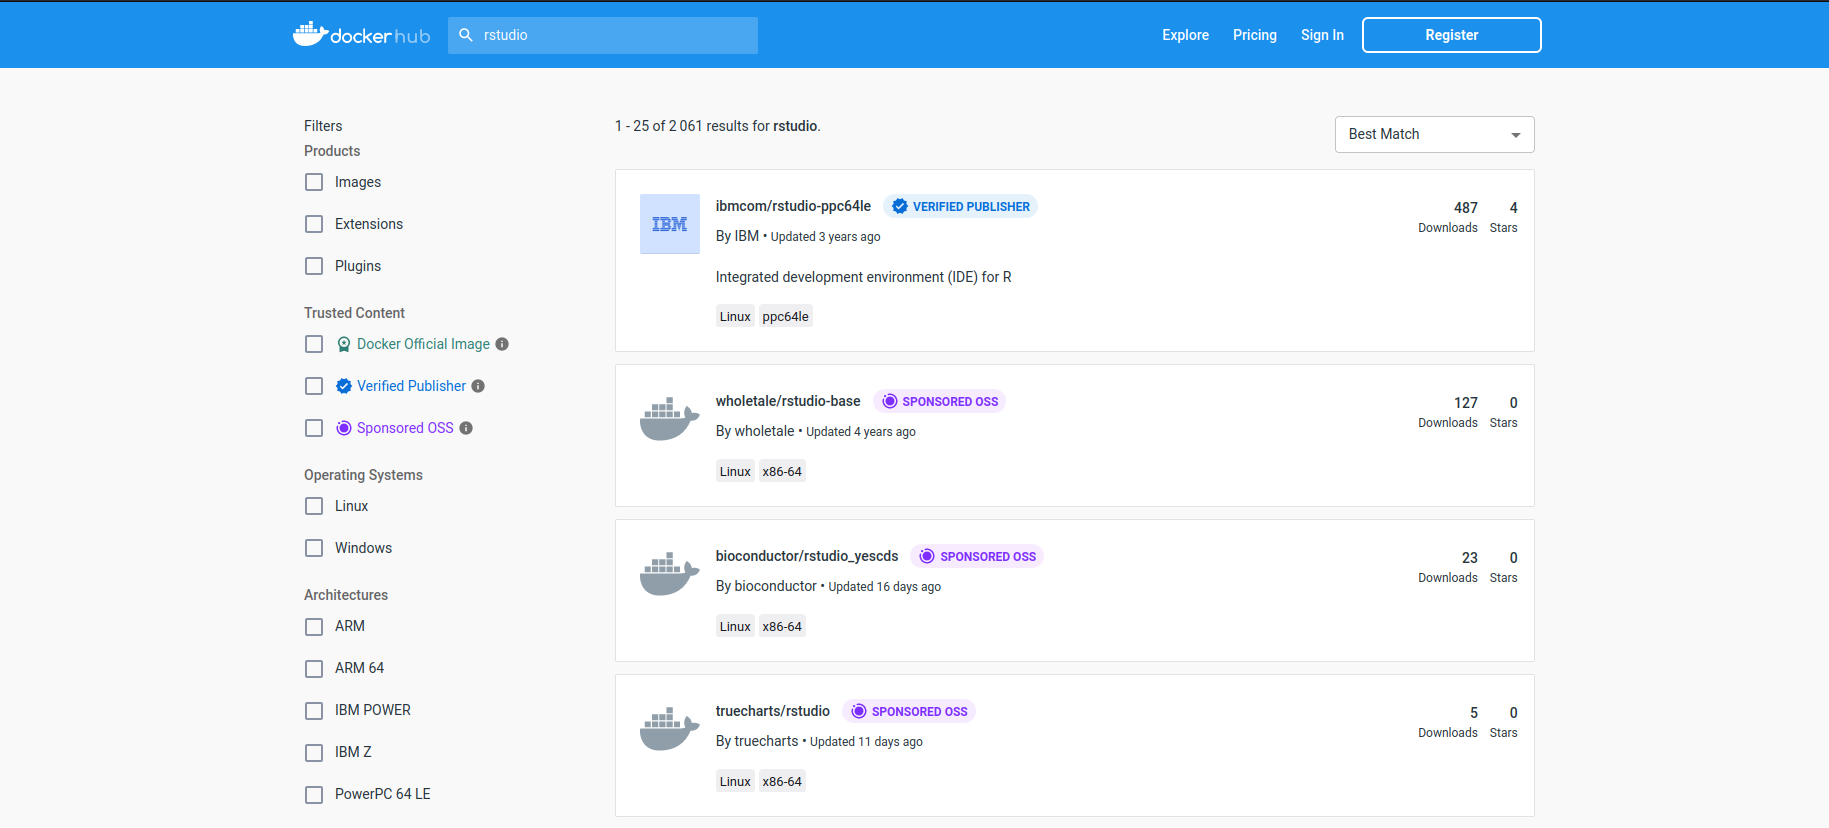
\includegraphics[width=0.1\textwidth]{images/docker_hub.png} 
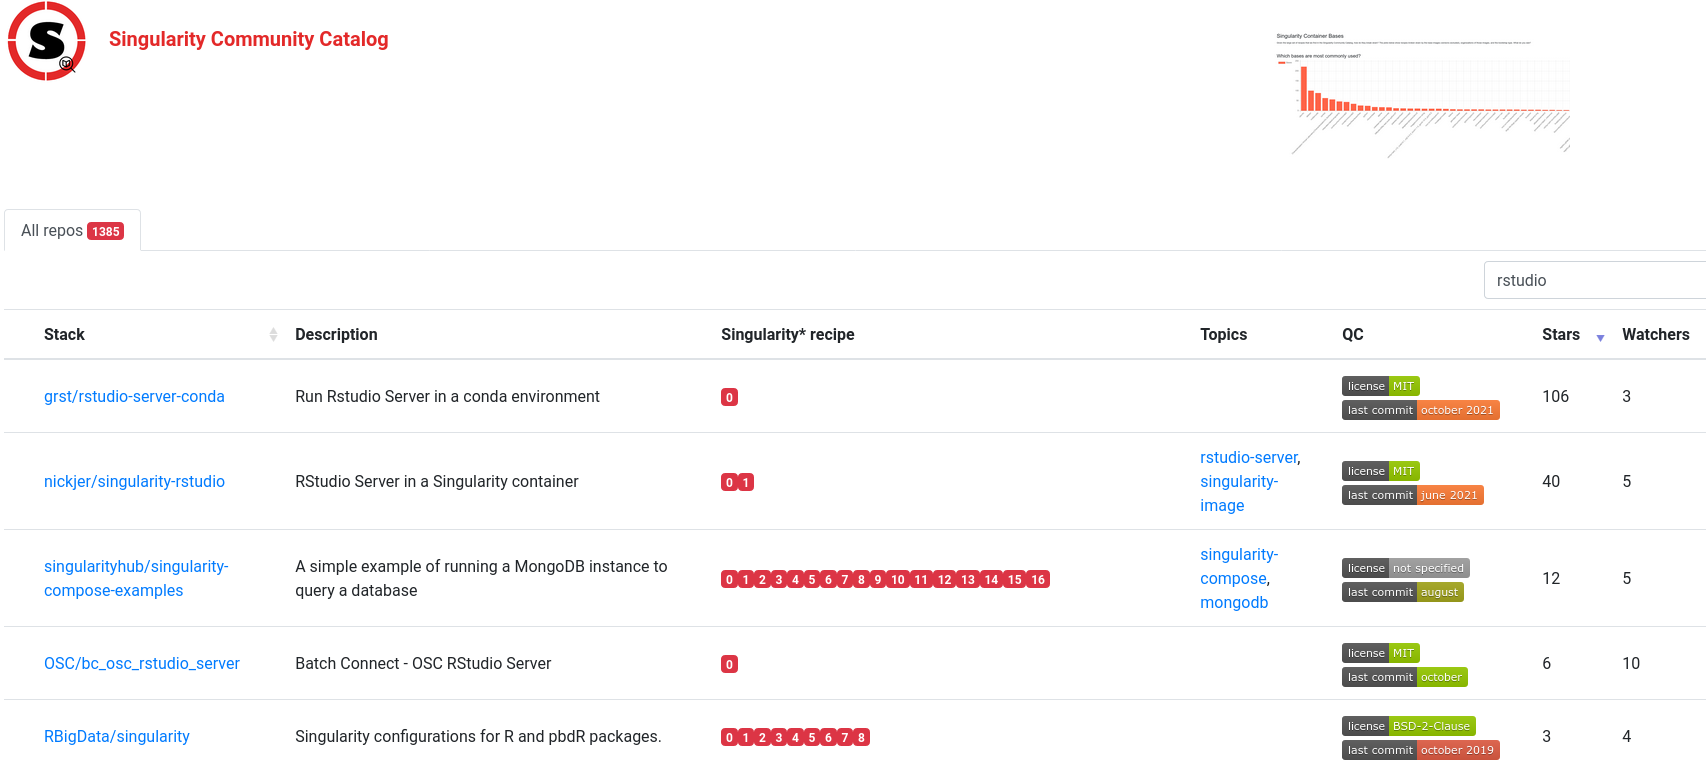
\includegraphics[width=0.1\textwidth]{images/singularity_hub.png}
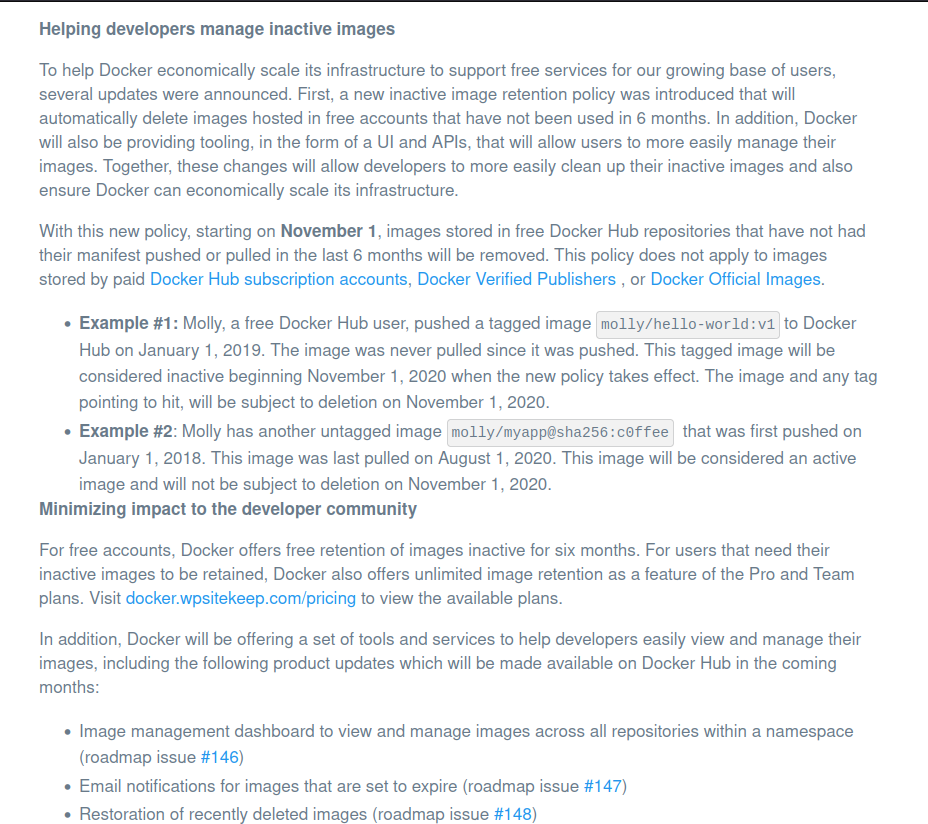
\includegraphics[width=0.1\textwidth]{images/docker_retention.png}
\footnote{\url{https://www.docker.com/blog/scaling-docker-to-serve-millions-more-developers-network-egress/}}
\end{frame}